\begin{mainquestion}{ammeter}{Equivalent Circuits}
Consider the circuit shown below. An ammeter with an internal resistance of $R_{i}$ is used to measure the current flowing through a \qty{560}{\ohm} resistor between points $A$ and $B$.

\begin{center}
    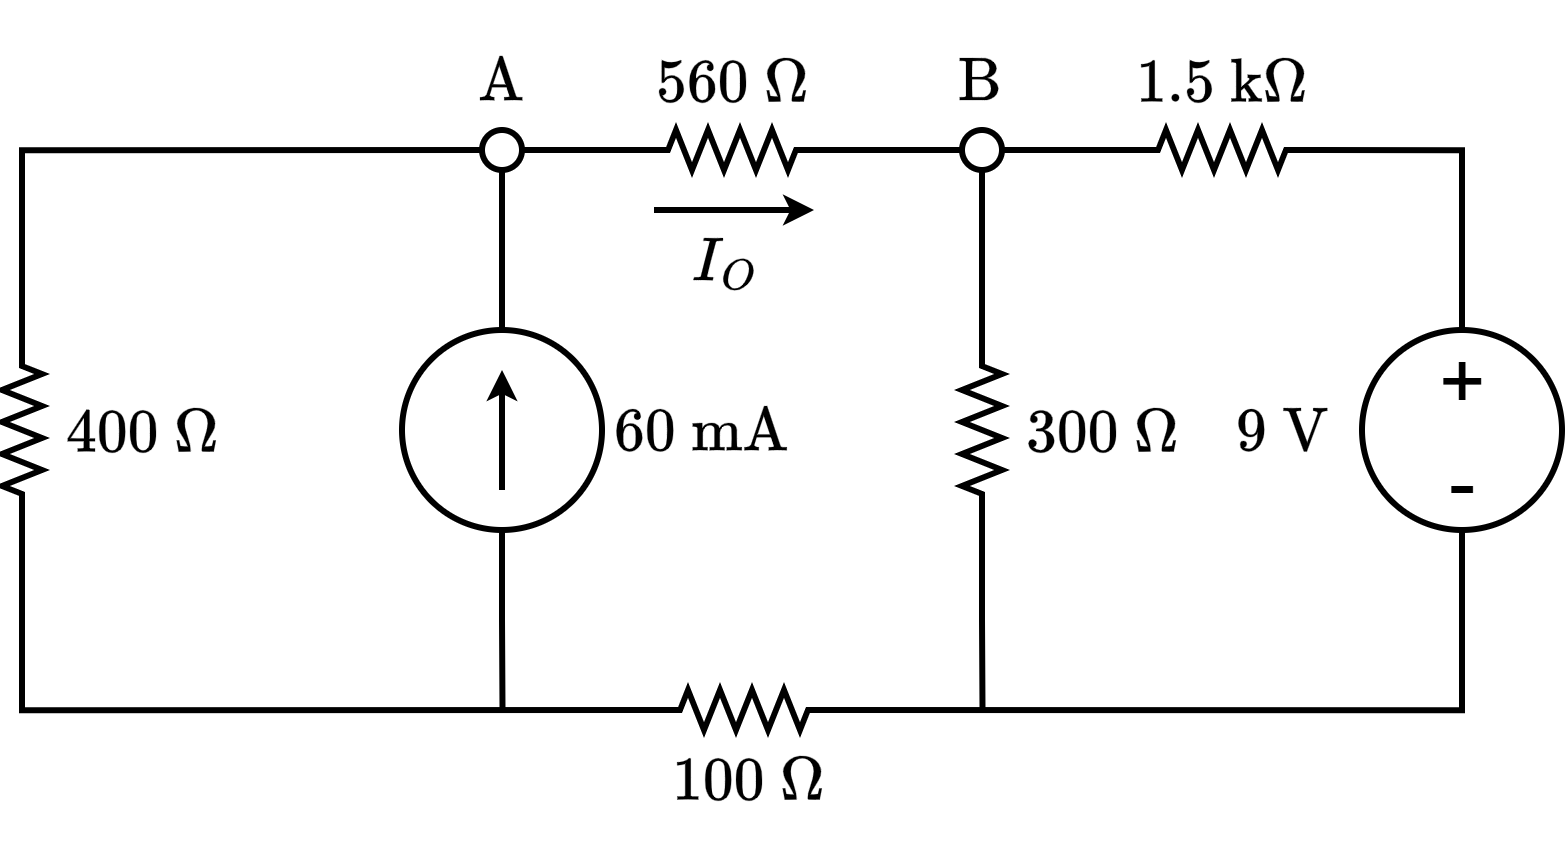
\includegraphics[width=5in]{circuit.png}
\end{center}

\begin{partquestion}{connection}{How should the ammeter be connected between $A$ and $B$? Show a sketch of the circuit (only include the portion between $A$ and $B$) which includes the ammeter with its internal resistance.}
\begin{answer}
The ammeter should be connected in series with the \qty{560}{\ohm} resistor between terminals $A$ and $B$. This means the current through the load passes through the ammeter and its internal resistance.

\begin{center}
    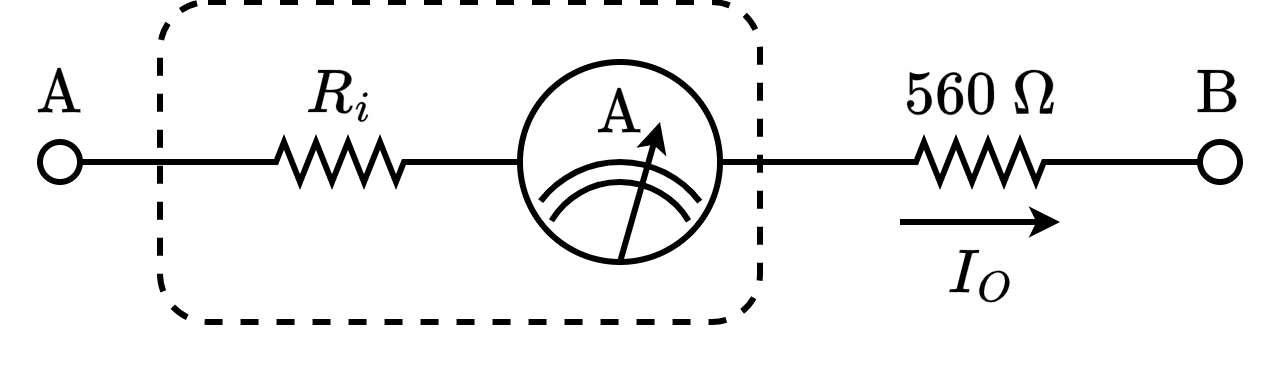
\includegraphics[width=0.7\textwidth]{ammeter_conn.png}
\end{center}
\end{answer}
\end{partquestion}

\begin{partquestion}{thevenin}{Find the Thévenin equivalent circuit at terminals $A$ and $B$ (without the \qty{560}{\ohm} load).}
\begin{answer}
To find the Thévenin resistance, we zero out all independent sources. The current source becomes an open circuit and the voltage source becomes a short circuit:

\begin{center}
    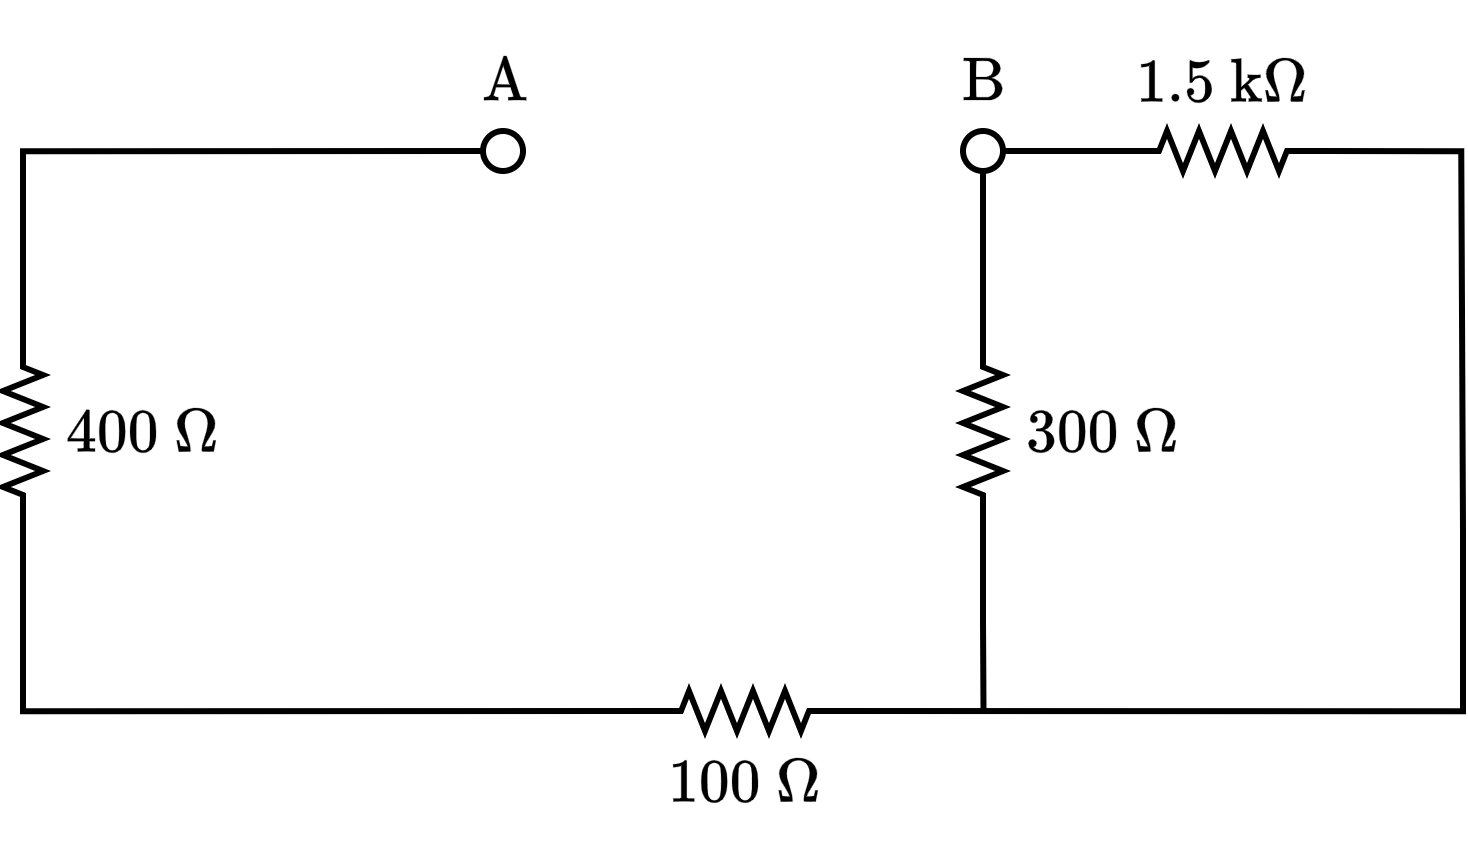
\includegraphics[width=0.7\textwidth]{rthev.png}
\end{center}

We can now combine the remaining resistors to find a single equivalent resistance.

\begin{align*}
    R_{TH} &= \qty{400}{\ohm} + \qty{100}{\ohm} + \qty{300}{\ohm}||\qty{1.5}{\kilo\ohm} \\
    &= \qty{500}{\ohm} + \frac{0.3\cdot1.5}{0.3+1.5}\unit{\kilo\ohm} \\
    &= \qty{750}{\ohm} \\
\end{align*}

\begin{center}
    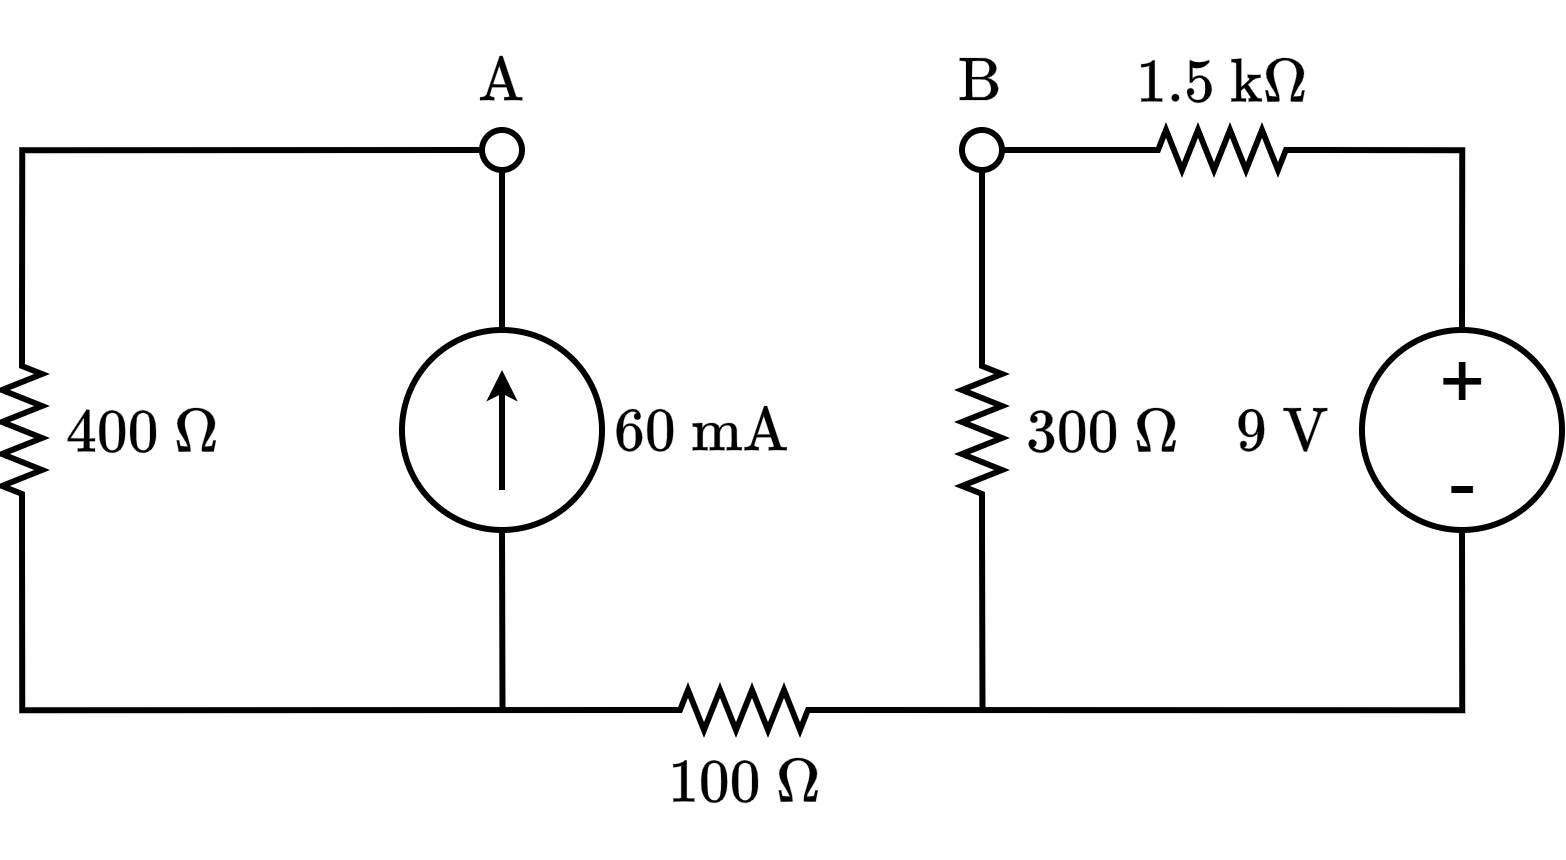
\includegraphics[width=4.5in]{thev_start.png}
\end{center}

Now to find the Thévenin voltage, compute the open-circuit voltage at $A$ and $B$. Because no current flows through the \qty{100}{\ohm} branch, its voltage is zero. The open-circuit voltage measured from $A$ to $B$ is therefore the voltage drop across the current source ($\qty{60}{\milli\ampere} \cdot\qty{400}{\ohm} = \qty{24}{\volt}$) minus the output of the voltage divider formed from the \qty{1.5}{\kilo\ohm} and \qty{300}{\ohm} resistors with the 9 V source ($9 \frac{3}{3+15} = \qty{1.5}{\volt}$). Thus $V_{\text{TH}} = 24 - 1.5 = \qty{22.5}{\volt}$.

Now that we have both the Thévenin voltage and Thévenin resistance, we can combine them to find our equivalent circuit:

\begin{center}
    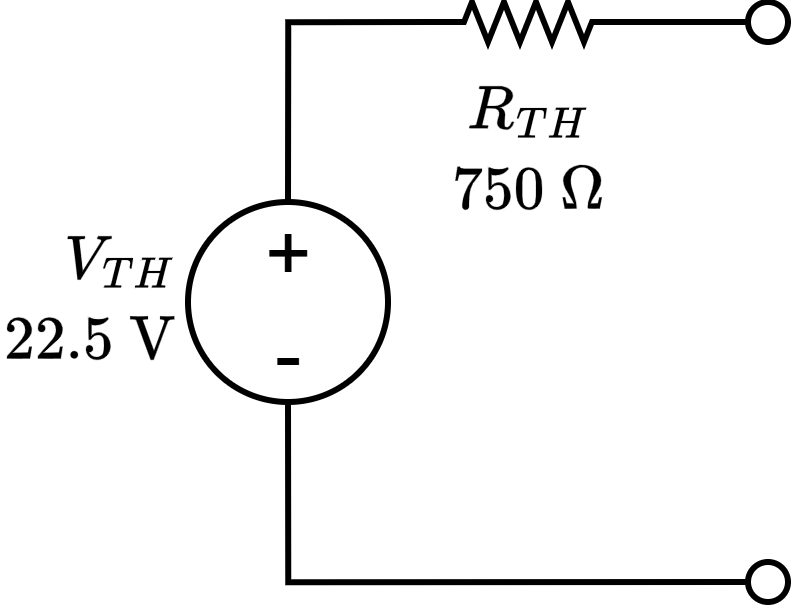
\includegraphics[width=2in]{thev_eq.png}
\end{center}
\end{answer}
\end{partquestion}

\begin{partquestion}{norton}{Find the Norton equivalent circuit at terminals $A$ and $B$ (without the \qty{560}{\ohm} load).}
\begin{answer}
Using the previously computed Thévenin equivalent, the Norton current is $I_{N} = V_{\text{TH}} / R_{\text{TH}} = \qty{22.5}{\volt} / \qty{750}{\ohm} = \qty{30}{\milli\ampere}$, and $R_{N} = \qty{750}{\ohm}$.

\begin{center}
    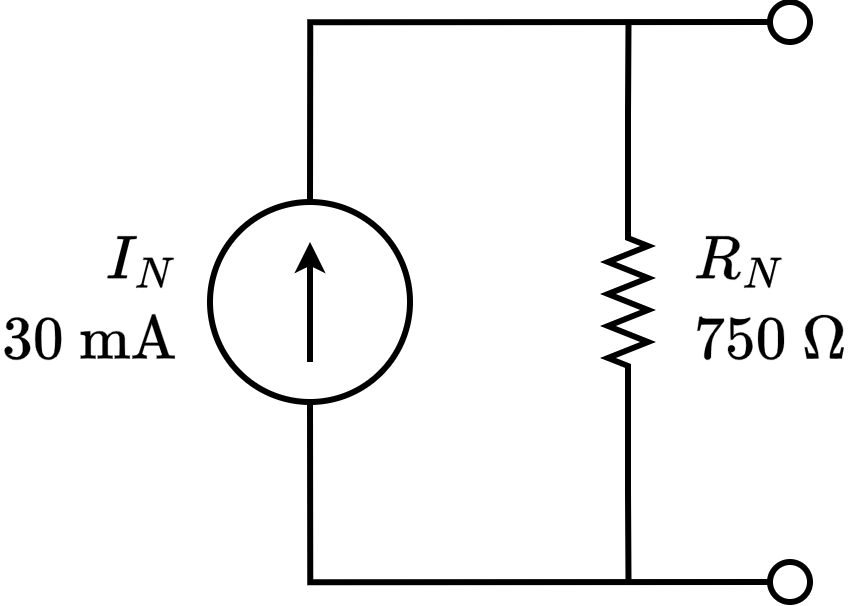
\includegraphics[width=2.2in]{norton_eq.png}
\end{center}
\end{answer}
\end{partquestion}

\begin{partquestion}{ri300}{What is the ammeter reading if $R_{i}=\qty{90}{\ohm}$?}
\begin{answer}
Using the Thévenin equivalent with $R_{i}=\qty{90}{\ohm}$ and $R_{L}=\qty{560}{\ohm}$ gives:
\[
I_O = \frac{V_{\text{th}}}{R_{\text{th}} + R_{i} + R_{L}} = \frac{22.5}{750 + 90 + 560} \approx \qty{16.07}{\milli\ampere}.
\]
\end{answer}
\end{partquestion}

\begin{partquestion}{ri0}{What is the ammeter reading if $R_{i}=\qty{0}{\ohm}$?}
\begin{answer}
With $R_{i}=\qty{0}{\ohm}$ the current is:
\[
I_O = \frac{22.5}{750 + 0 + 560} \approx \qty{17.17}{\milli\ampere}.
\]
\end{answer}
\end{partquestion}

\begin{partquestion}{rimax}{What is the maximum value of $R_{i}$ such that the deviation in $I_O$ is less than 1\%? Find the ammeter reading with this maximum.}
\begin{answer}
Let's call the max deviation $\alpha = 0.01$. Since adding any $R_i$ reduces the total current, we wish to determine when $I_{R_i}/I_{0} \geq 1-\alpha$. Let's solve for $R_i$:
\begin{align*}
    \frac{I_{R_i}}{I_0} &\geq 1-\alpha \\
    \frac{R_{th} + R_L}{R_{th} + R_L + R_i} &\geq 1-\alpha \\
    \frac{R_{th} + R_L}{1-\alpha} &\geq R_{th} + R_L + R_i \\
    (R_{th} + R_L)(\frac{1}{1-\alpha} - 1) &\geq R_i \\
    R_i &\leq (R_{th} + R_L)\frac{\alpha}{1-\alpha} \\
    R_i &\leq (750 + 560)\frac{0.01}{0.99} \\
    R_i &\leq 13.23\unit{\ohm}
\end{align*}

Let's find $I_O$ with this new resistance:
\[
I_O = \frac{22.5}{750 + 13.23 + 560} \approx 17.00~\text{mA (nice)}
\]

\end{answer}
\end{partquestion}

\end{mainquestion}
